\documentclass{beamer}

%\usetheme{Goettingen}
%\usetheme{Berkeley}
%\usetheme{Boadilla}
%\usetheme{Copenhagen}

\usepackage[math]{iwona}
\usepackage{graphicx}
\usepackage{wrapfig}
\usepackage{pgf,tikz}
\usetikzlibrary{shapes.gates.logic.US,trees,positioning,arrows}
\usepackage{hyperref}
\usepackage{float}
\hypersetup{colorlinks=true}

\usepackage[utf8]{inputenc}
\usepackage[spanish]{babel}


\title[Taller de \LaTeX]{Inserci\'on de gr\'aficos en \LaTeX}
\author[O. S\'anchez]{}
\institute[UGR]{Universidad de Granada}
\date{\today}
\begin{document}

\maketitle

\section{Formatos gr\'aficos}
\begin{frame}{Generalidades sobre formatos gr\'aficos}
\begin{block}{Mapas de bits} 
\begin{center}
\includegraphics[width=7cm]{./graficos/QtOctave.pdf}
\end{center}
Extensiones: BMP, JPEG, GIF, PNG y TIFF. \\
{\small Desventaja: deformaciones al reescalar y gran tama\~no.}
\end{block}
\end{frame}
\begin{frame}
\begin{block} {Gr\'aficos vectoriales} 
\begin{center}
\includegraphics[width=7cm]{graficos/fplot.pdf}
\end{center}
Extensiones: EPS, PDF, SVG, WMF \\
{\small Nota: !`Estos archivos pueden insertar mapas de bits! }
\end{block}
\end{frame}

%%%%%%%%%%%%%%%%%%%%%%%%%%%%%%%%%%%%%%%%

\begin{frame}{Preparaci\'on de gr\'aficos para insertar en \LaTeX}
El formato del gr\'afico a insertar depende del compilador empleado:
\begin{enumerate}
\item \it{latex + dvips}  se requiere PS / EPS {\scriptsize(con \href{http://tex.stackexchange.com/questions/133786/no-boundingbox-error-message}{BoundingBox})}
\item \it {pdflatex} se requiere PNG {\scriptsize(mapas de bits simples)}, JPEG {\scriptsize(fotograf\'ias)} o PDF {\scriptsize(gr\'aficos vectoriales)}
\end{enumerate}

\vspace{0.5cm}
Esto requiere de programas espec\'ificos de transformaci\'on:
\begin{itemize}
\item {\sc EPS a PDF}: \href{http://tug.org/epstopdf/}{epstopdf}
%\item {\sc JPEG a EPS}: \href{http://www.pdflib.com/download/free-software/jpeg2ps/}{jpeg2ps}
\item {\sc Todo a Todo}: \href{http://www.inkscape.org/es/}{Inkscape}, 
\href{http://www.imagemagick.org}{ImageMagick} o \href{http://www.gimp.org/}{Gimp}
\item ........
\end{itemize}
Nosotros nos centramos en c\'omo generar gr\'aficos con programas de matem\'aticas aunque se puede incluir 
cualquier tipo de gr\'afico.
\end{frame}

%%%%%%%%%%%%%%%%%%%%%%%%%%%%%%%%%%%%%%%%

\begin{frame}{Paquetes matem\'aticos con los que generar gr\'aficos}
Hay una gran variedad de  paquetes matem\'aticos que podemos emplear para generar ficheros 
gr\'aficos:
\begin{enumerate}
\item Octave
\item Sage  (Gnuplot)
\item Maxima (Gnuplot)
\item Mathematica {\small (problemas de fuentes!!!)}
\item Matlab
\item y un largo etc...
\end{enumerate}

Se puede ver un listado exhaustivo en \href{https://en.wikibooks.org/wiki/LaTeX/Importing_Graphics\#Third-party_graphics_tools}{el siguiente wikibook}.

\end{frame}

%%%%%%%%%%%%%%%%%%%%%%%%%%%%%%%%%%%%%%%%%%
\section{Inserci\'on de un gr\'afico}
\begin{frame}[fragile]{Insertar el gr\'afico como una figura}
Declaraci\'on del paquete graphicx en el pre\'ambulo:
\begin{verbatim}\usepackage{graphicx} \end{verbatim}

Inserci\'on del gr\'afico en el documento:
\begin{verbatim}
\begin{figure}
  \centering
  \includegraphics[parametros]{nombregrafico}
  \caption{Leyenda bajo el grafico}
  \label{fig:etiqueta}
\end{figure}
\end{verbatim}
Mediante los par\'ametros se puede modificar el aspecto:\\
\begin{verbatim}height=0.5\textwidth, keepaspectratio,angle=90, ....\end{verbatim}
Para profundizar ver documentaci\'on paquete graphicx \cite{DocGraphicx} .
\end{frame}
%%%%%%%%%%%%%%%%%%%%%%%%%%%%%%%%%%%%%%%%%%%%
\begin{frame}[fragile]
\begin{exampleblock}{Ejercicio 1: Inserta un gr\'afico entre texto}
{\small As\'i el comando de Octave\\
\verb|>> t = 0:0.2:6.3;  plot (t, sin(t),'-@r*;sin(t);')|
representa la funci\'on seno variando dichas propiedades
\begin{figure}
\begin{center}
\includegraphics[width=0.45\textwidth]{graficos/sin.pdf}
\end{center}
\caption{Gr\'afico con estilo \label{figura:sinestilo}}
\end{figure}
tras lo cual se guarda en un fichero  en formato EPS o PDF.
Este fichero gr\'afico se puede insertar en un documento \LaTeX como en la figura \ref{figura:sinestilo}.
}
\end{exampleblock}
\end{frame}

%%%%%%%%%%%%%%%%%%%%%%%%%%%%%%%%%%%%%%%%%%%%%

\begin{frame}[fragile]
\begin{exampleblock}{Soluci\'on: Inserci\'on de un gr\'afico}

\begin{verbatim}
As\'i el comando de Octave\\
\verb|>> t = 0:0.2:6.3;  plot (t, sin(t),'-@r*;sin(t);')|
representa la funci\'on seno variando dichas propiedades
\begin{figure}
\begin{center}
\includegraphics[width=0.45\textwidth]{graficos/sin.pdf}
\end{center}
\caption{Gr\'afico con estilo \label{figura:sinestilo}}
\end{figure}
tras lo cual se guarda en un fichero en formato EPS o PDF.
Este fichero gr\'afico se puede insertar en un documento 
\LaTeX como en la figura \ref{figura:sinestilo}
\end{verbatim}
\end{exampleblock}
\end{frame}

%%%%%%%%%%%%%%%%%%%%%%%%%%%%%%%%%%%%%%%%%%

\begin{frame}[fragile]{Modificaci\'on de la imagen}
\LaTeX $ $ permite modificar mediante par\'ametros el aspecto de la figura insertada.\\
\verb|[ trim = 10mm 5mm 50mm 55mm, clip,width=0.6\textwidth]|
\verb| %trim = <left> <lower> <right> <upper> |
\begin{figure}
\begin{center}
\includegraphics[trim = 10mm 5mm 50mm 55mm, clip,width=0.6\textwidth]{graficos/sin.pdf}

\end{center}
\caption{Gr\'afico recortado y ampliado \label{figura:sinestilo}}
\end{figure}

\end{frame}

%%%%%%%%%%%%%%%%%%%%%%%%%%%%%%%%%%%%%%%%%%

\begin{frame}[fragile]{El posicionamiento del entorno figure}
\LaTeX posiciona la figura que se ha declarado dentro de un entorno figure en el sitio que estima
mejor seg\'un su criterio, que puede no coincidir con el nuestro.

Para forzar al entorno a situarse en un lugar concreto se puede declarar el paquete 
float en el pre\'ambulo:\\
\verb|\usepackage{float}|\\
y a\~nadir el modificador [H] al entorno figure:
\begin{verbatim}
\begin{figure}[H]
\begin{center}
\includegraphics[width=0.45\textwidth]{graficos/sin.pdf}
\end{center}
\caption{Gr\'afico con estilo \label{figura: forzada}}
\end{figure}
\end{verbatim}
Tienes m\'as informaci\'on en el siguiente \href{http://ltx.blogspot.com.es/2003/10/quiero-mi-figura-aqui.html}{blog: \LaTeX $ $  y compa\~nia}
\end{frame}

%%%%%%%%%%%%%%%%%%%%%%%%%%%%%%%%%%%%%%%%%%

\begin{frame}[fragile]{El paquete wrapfig}
Otra opci\'on es integrar el gr\'afico con el texto empleando el paquete  \href{http://www.ctan.org/pkg/wrapfig}{wrapfig}
\vskip 12pt
Declaraci\'on del paquete wrapfig en el pre\'ambulo:
\begin{verbatim} \usepackage{wrapfig} \end{verbatim}

Inserci\'on del gr\'afico en el documento:
\begin{verbatim}
\begin{wrapfigure}{r}{<width>}
  \includegraphics[parametros]{nombregrafico}
  \caption{Leyenda bajo el grafico}
  \label{fig:etiqueta}
\end{wrapfigure}
\end{verbatim}
\end{frame}


%%%%%%%%%%%%%%%%%%%%%%%%%%%%%%%%%%%%%%%%%%%%
\begin{frame}[fragile]
\begin{exampleblock}{Ejercicio 2: Inserci\'on de un gr\'afico con wrapfigure}
{\small As\'i el comando
\\%%
\verb|>> t = 0:0.2:6.3;  plot (t, sin(t),'-@r*;sin(t);')|
representa la funci\'on seno variando dichas propiedades.
Una vez generado el gr\'afico, se pueden a\~nadir t\'itulos, etiquetas a los ejes, mallados o incluso redimensionar la figura
tal y como indican los siguientes comandos:\\%%
\begin{wrapfigure}{r}{0.5\textwidth}
\begin{center}
\vspace{-30pt}
\includegraphics[width=5cm]{graficos/sin.pdf}
  \end{center}
\vspace{-25pt}
  \caption{{\tiny Gr\'afico con estilo \label{figura:sinestilo1}}}
\end{wrapfigure}
\verb|>> title('Grafico de Sen(t)')|
\\%%
\verb|>> xlabel('Angulo')|
\\%%
\verb|>> ylabel('sin(t)')|
\\%%
\verb|>> grid on|
\\%%

Para guardar un gr\'afico en formatos EPS o PDF se puede emplear el comando print de la siguiente manera:
\\
\verb|>> print('grafico1.eps','-deps')| \\
\verb|>> print('grafico1.pdf ','-dpdf')| \\
dango lugar al gr\'afico que presentamos en la fig. \ref{figura:sinestilo1}.
}
\end{exampleblock}
\end{frame}

%%%%%%%%%%%%%%%%%%%%%%%%%%%%%%%%%%%%%%%%%%%%%%%%%%%%

\begin{frame}[fragile]
\begin{exampleblock}{Soluci\'on: Inserci\'on de un gr\'afico con wrapfigure}

\begin{verbatim}
\begin{wrapfigure}{r}{0.5\textwidth}
\begin{center}
\vspace{-30pt}
\includegraphics[width=5cm]{graficos/sin.pdf}
\end{center}
\vspace{-25pt}
\caption{{\tiny Gr\'afico con estilo}}
\label{figura:sinestilo1}
\end{wrapfigure}
\end{verbatim}

{\small {\color{red} ADVERTENCIA:} Puede requerir de ajuste de espaciado superior e inferior para dejarlo a tu gusto... }

\end{exampleblock}
\end{frame}




%%%%%%%%%%%%%%%%%%%%%%%%%%%%%%%%%%%%%%%%%%%%%%%%%%%%
\begin{frame}[fragile]
\begin{exampleblock}{Ejercicio 3: Inserci\'on de varios gr\'aficos}
Se pueden introducir simult\'aneamente varios gr\'aficos en un mismo entorno 
figure para que aparezcan juntos siempre que el tama\~no lo permita.
\begin{figure}
\includegraphics[width=4.5cm]{./graficos/sorpresa}
\hspace{0.5cm}
\reflectbox{
\includegraphics[width=4.5cm]{./graficos/sorpresa}}
\caption{La misma imagen reflejada.}
\end{figure}
\end{exampleblock}
\end{frame}

%%%%%%%%%%%%%%%%%%%%%%%%%%%%%%%%%%%%%%%%%%%%%%%%%%%%
\begin{frame}[fragile]
\begin{exampleblock}{Soluci\'on: Inserci\'on de varios gr\'aficos}
Se pueden introducir simult\'aneamente varios gr\'aficos en un mismo entorno 
figure para que aparezcan juntos siempre que el tama\~no lo permita.
\begin{verbatim}
\begin{figure}
\includegraphics[width=4.5cm]{./graficos/sorpresa}
\hspace{0.5cm}
\reflectbox{
\includegraphics[width=4.5cm]{./graficos/sorpresa}
}
\caption{La misma imagen reflejada.}
\end{figure}
\end{verbatim}
\end{exampleblock}
\end{frame}

%%%%%%%%%%%%%%%%%%%%%%%%%%%%%%%%%%%%%%%%%%%%%%%%%%%%
\begin{frame}[fragile]
\begin{exampleblock}{Ejercicio 4: Superposici\'on de texto sobre gr\'aficos}
Mediante el comando \\
\verb|\put(coordenadas){objeto}|\\
se pueden superponer `el objeto' en la posicion `coordenadas'.
\begin{figure}
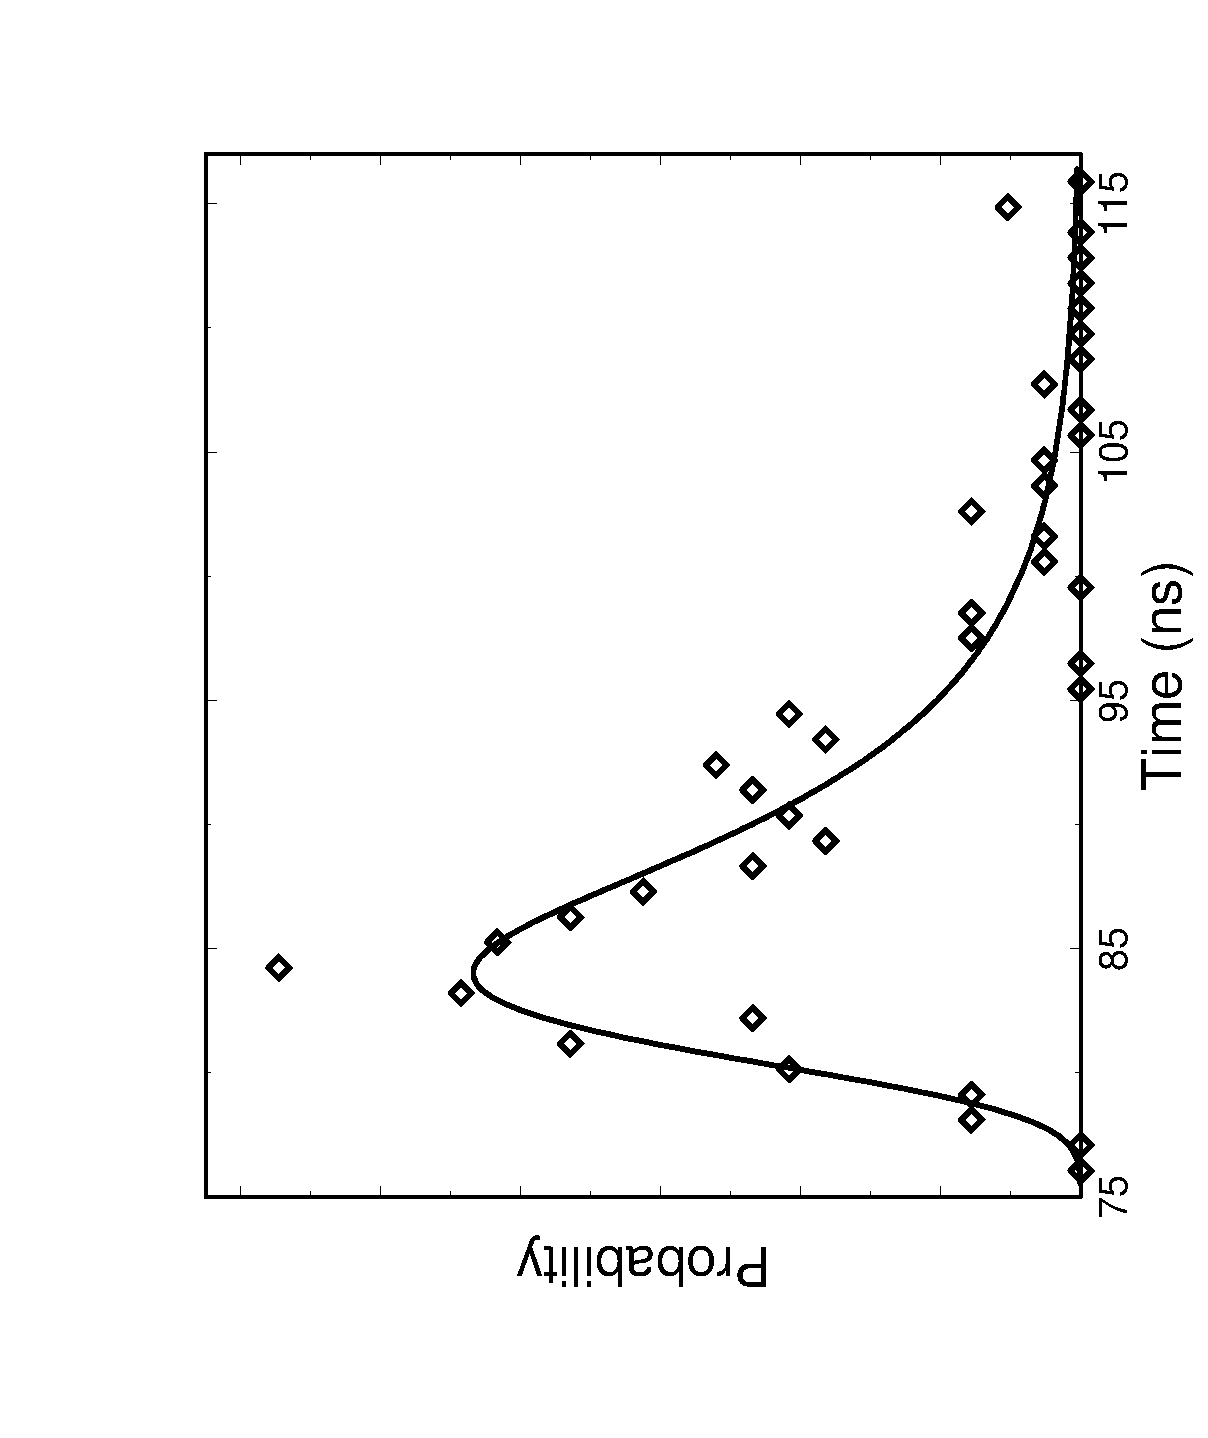
\includegraphics[angle=270,width=7cm]{./graficos/fig_9}
\put(-100,-55){$\displaystyle s:=\frac{a+b+c}{2}$}
\end{figure}
\end{exampleblock}
\end{frame}

%%%%%%%%%%%%%%%%%%%%%%%%%%%%%%%%%%%%%%%%%%%%%%%%%%%%
\begin{frame}[fragile]
\begin{exampleblock}{Soluci\'on: Superposici\'on de texto sobre gr\'aficos}
Mediante el comando \\
\verb|\put(coordenadas){objeto}|\\
se pueden superponer `el objeto' en la posicion `coordenadas'.

\begin{verbatim}
\begin{figure}
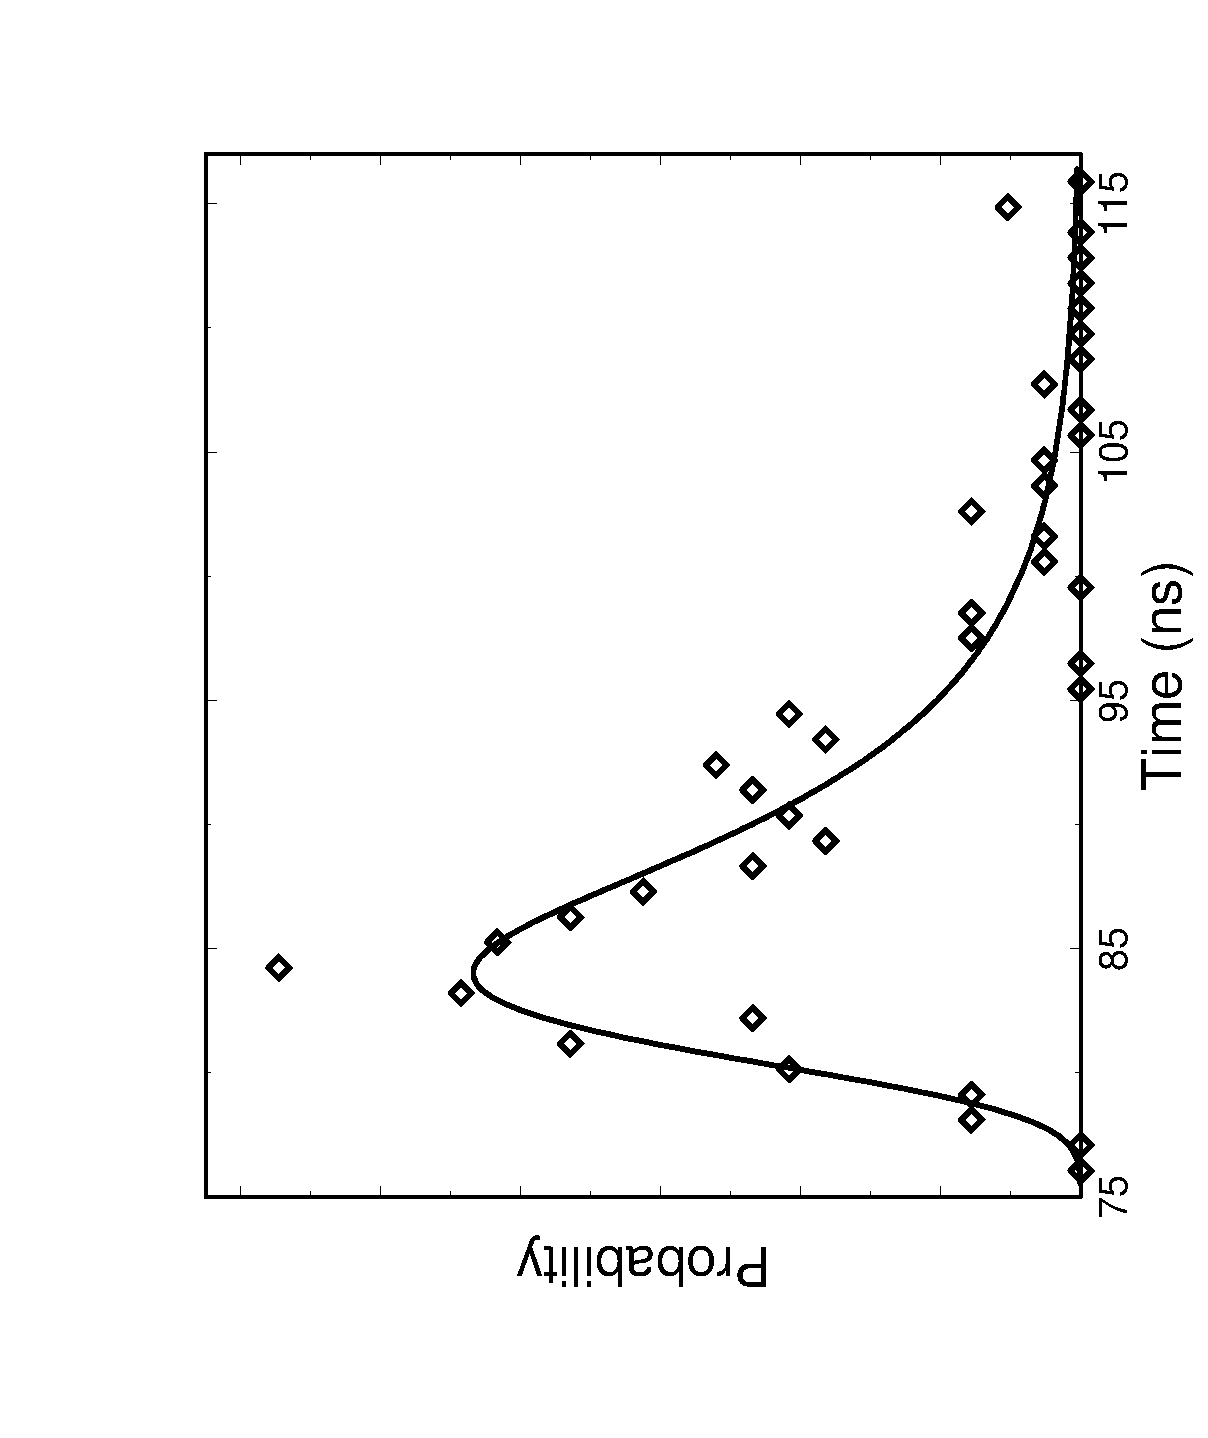
\includegraphics[angle=270,width=7cm]{./graficos/fig_9}
\put(-100,-55){$\displaystyle s:=\frac{a+b+c}{2}$}
\end{figure}
\end{verbatim}
\end{exampleblock}
\end{frame}

%%%%%%%%%%%%%%%%%%%%%%%%%%%%%%%%%%%%%%%%%%%%%%%%%%%%
\begin{frame}[fragile]
\begin{exampleblock}{Ejercicio 5: Superposici\'on de varios gr\'aficos}
{\scriptsize OJO!  Requiere  \href{https://docs.gimp.org/2.10/es/gimp-tutorial-quickie-separate.html}{fondo transparente} en la figura a superponer (objeto).}
%\includegraphics[angle=0, width=3cm]{./graficos/ciclista}
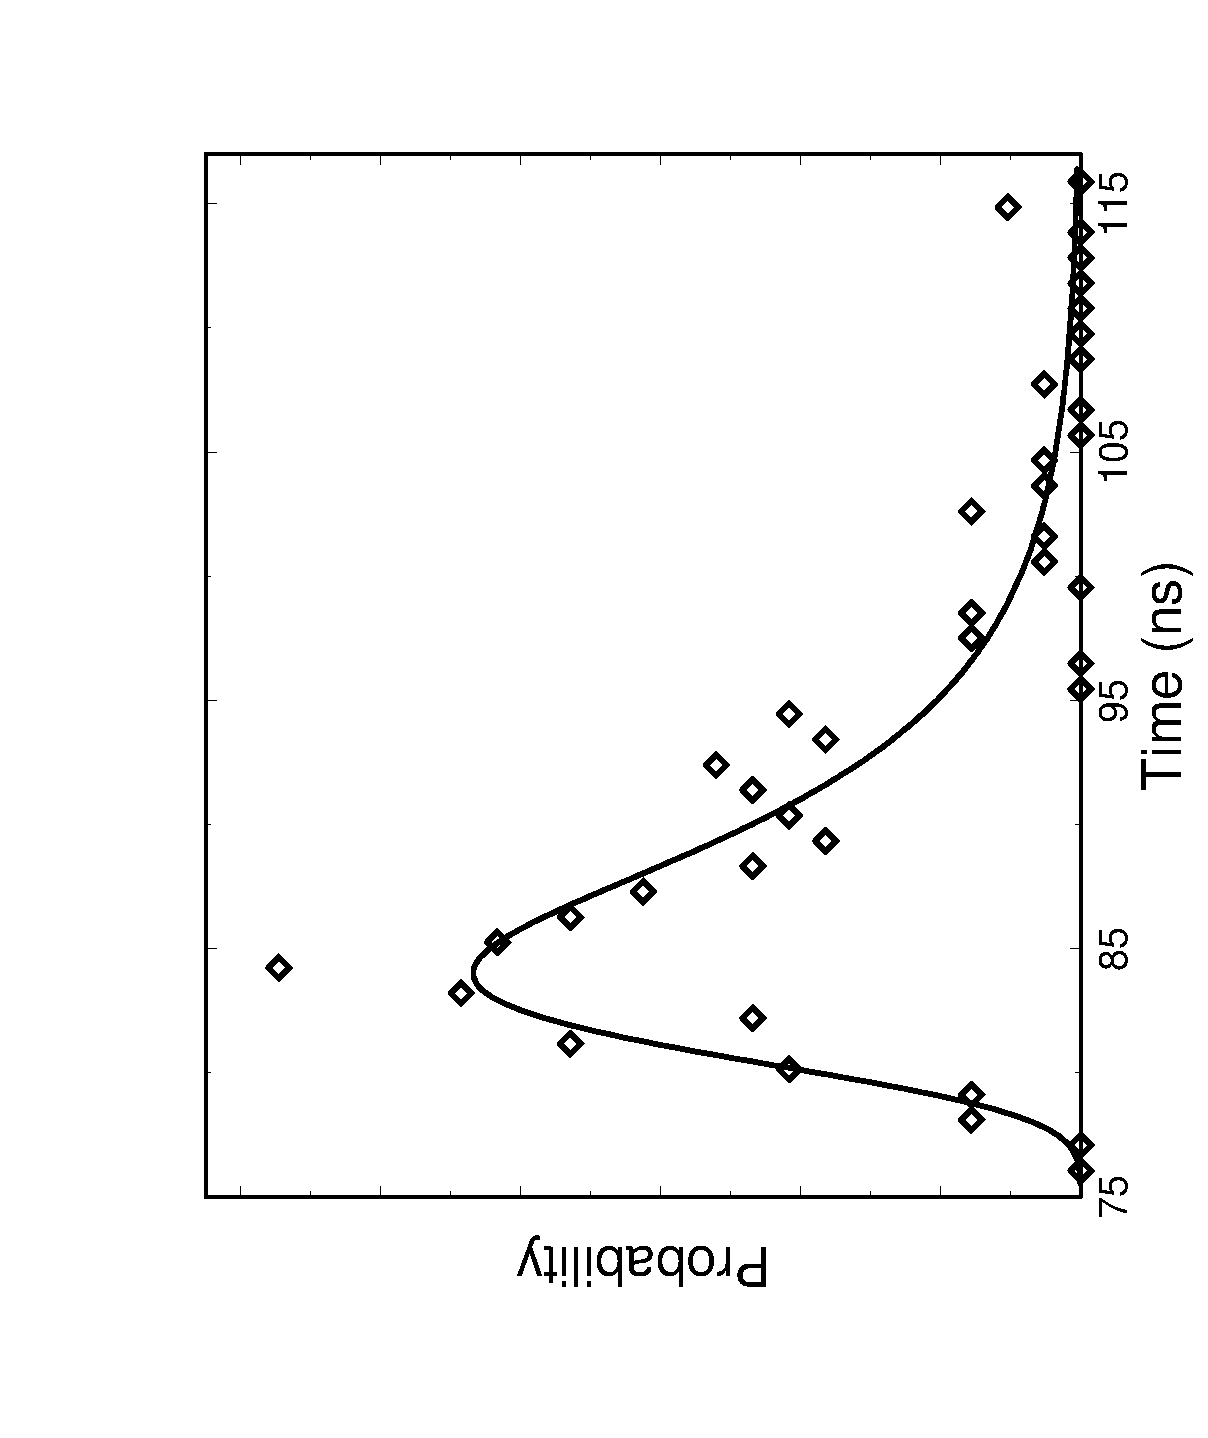
\includegraphics[angle=270,width=9cm]{./graficos/fig_9}
\put(-100,-205){\includegraphics[angle=-7,scale=0.4]{./graficos/ciclista}}
\end{exampleblock}
\end{frame}

%%%%%%%%%%%%%%%%%%%%%%%%%%%%%%%%%%%%%%%%%%%%%%%%%%%%
\begin{frame}[fragile]
\begin{exampleblock}{Soluci\'on: Superposici\'on de varios gr\'aficos}
{\scriptsize OJO!  Requiere  \href{https://docs.gimp.org/2.10/es/gimp-tutorial-quickie-separate.html}{fondo transparente} en la figura a superponer (objeto).}
\begin{verbatim}
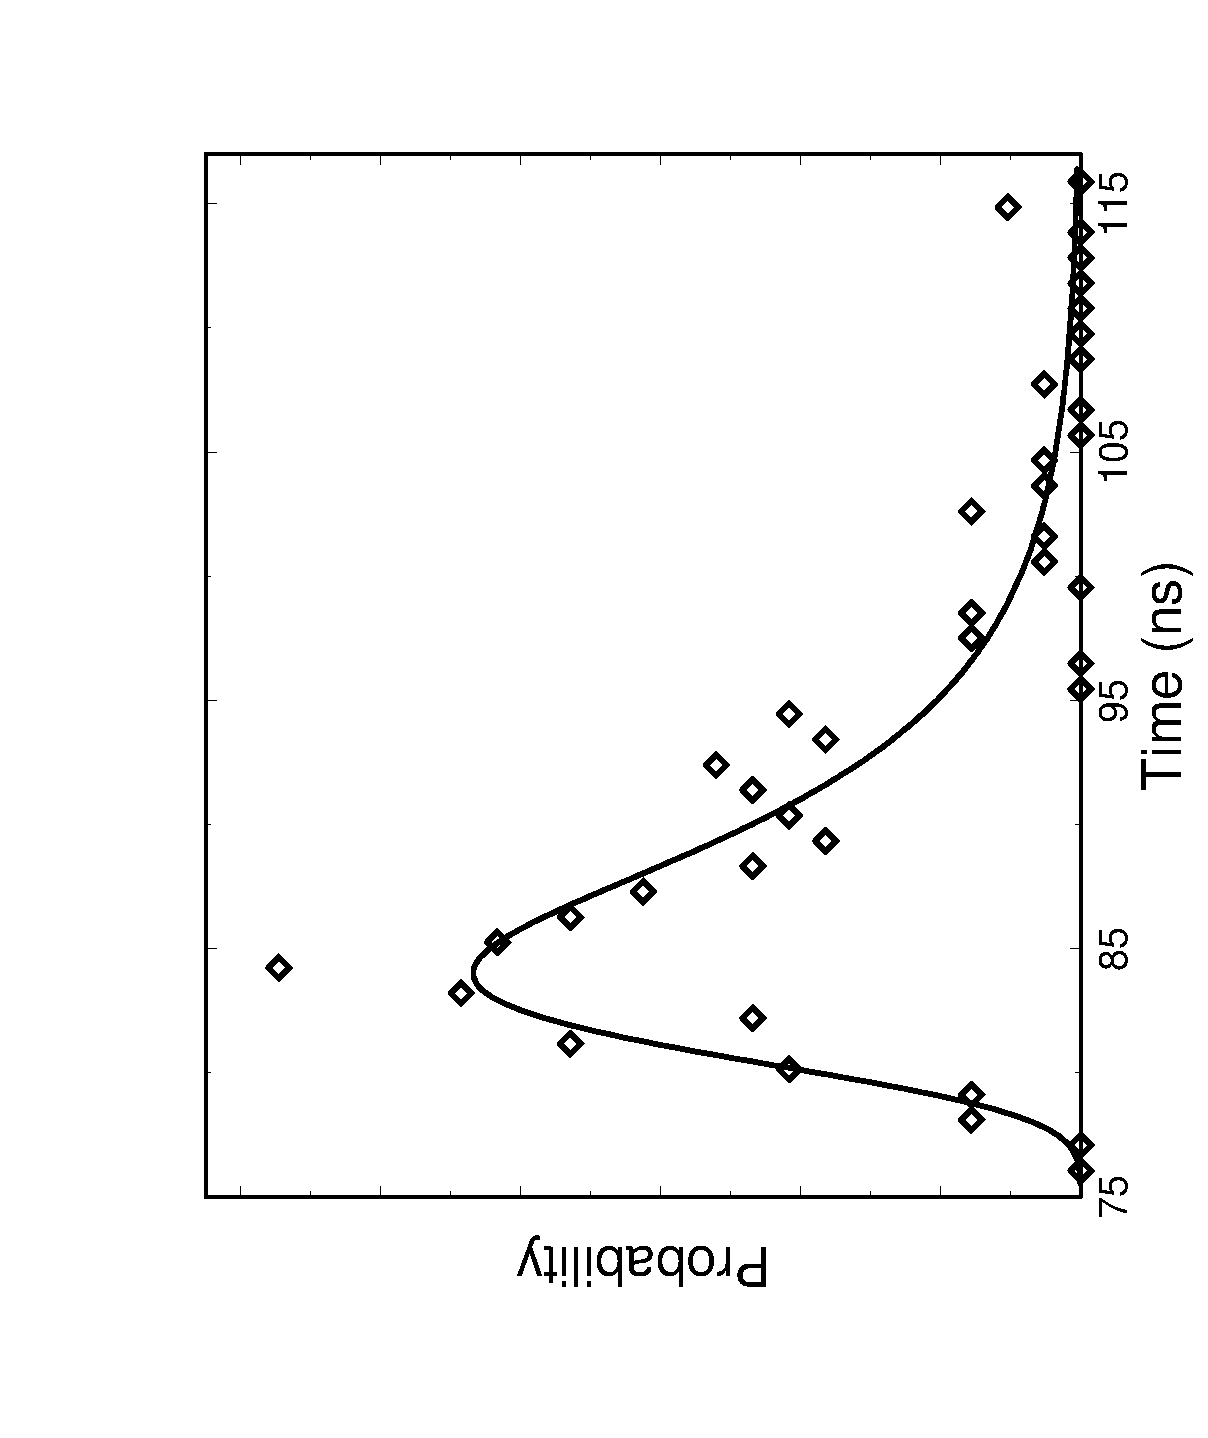
\includegraphics[angle=270,width=9cm]{./graficos/fig_9}
\put(-100,-205){
\includegraphics[angle=-7,scale=0.4]{./graficos/ciclista}
}
\end{verbatim}
\end{exampleblock}
\end{frame}

%%%%%%%%%%%%%%%%%%%%%%%%%%%%%%%%%%%%%%%%%%%%%
\begin{frame}[fragile]{Inserci\'on de figura generada con Xfig}
Existen programas, como \href{http://mcj.sourceforge.net}{Xfig} {\small (versi\'on shareware Windows: \href{http://winfig.com/}{WinFIG})}, 
que permiten hacer los diseños en un entorno gráfico y luego 
insertarlo con algunos elementos generados por \LaTeX .

\begin{verbatim}
\resizebox{7cm}{!}{\input ./graficos/deformacubos.pdf_t}
\end{verbatim}
\begin{center}
\resizebox{6cm}{!}{\input ./graficos/deformacubos.pdf_t}
\end{center}
\end{frame}

%%%%%%%%%%%%%%%%%%%%%%%%%%%%%%%%%%%%%%%%%%%%%
\begin{frame}[fragile]{Modificaci\'on de figura generada con Xfig}
Esta manera de insertar gr\'aficos tiene la ventaja de que aquellos elementos generados
por \LaTeX $ $ pueden ser f\'acilmente modificables, por ejemplo:

\begin{verbatim}
\resizebox{7cm}{!}{\input ./graficos/deformaMOD.pdf_t}
\end{verbatim}
\begin{center}
\resizebox{6cm}{!}{\input ./graficos/deformaMOD.pdf_t}
\end{center}
\end{frame}


%%%%%%%%%%%%%%%%%%%%%%%%%%%%%%%%%%%%%%%%%%%%%%%%%%%%
\begin{frame}[fragile]
\begin{exampleblock}{Ejercicio propuesto 1}
Insertar un subgr\'afico dentro de otro gr\'afico.
\end{exampleblock}
\begin{figure}
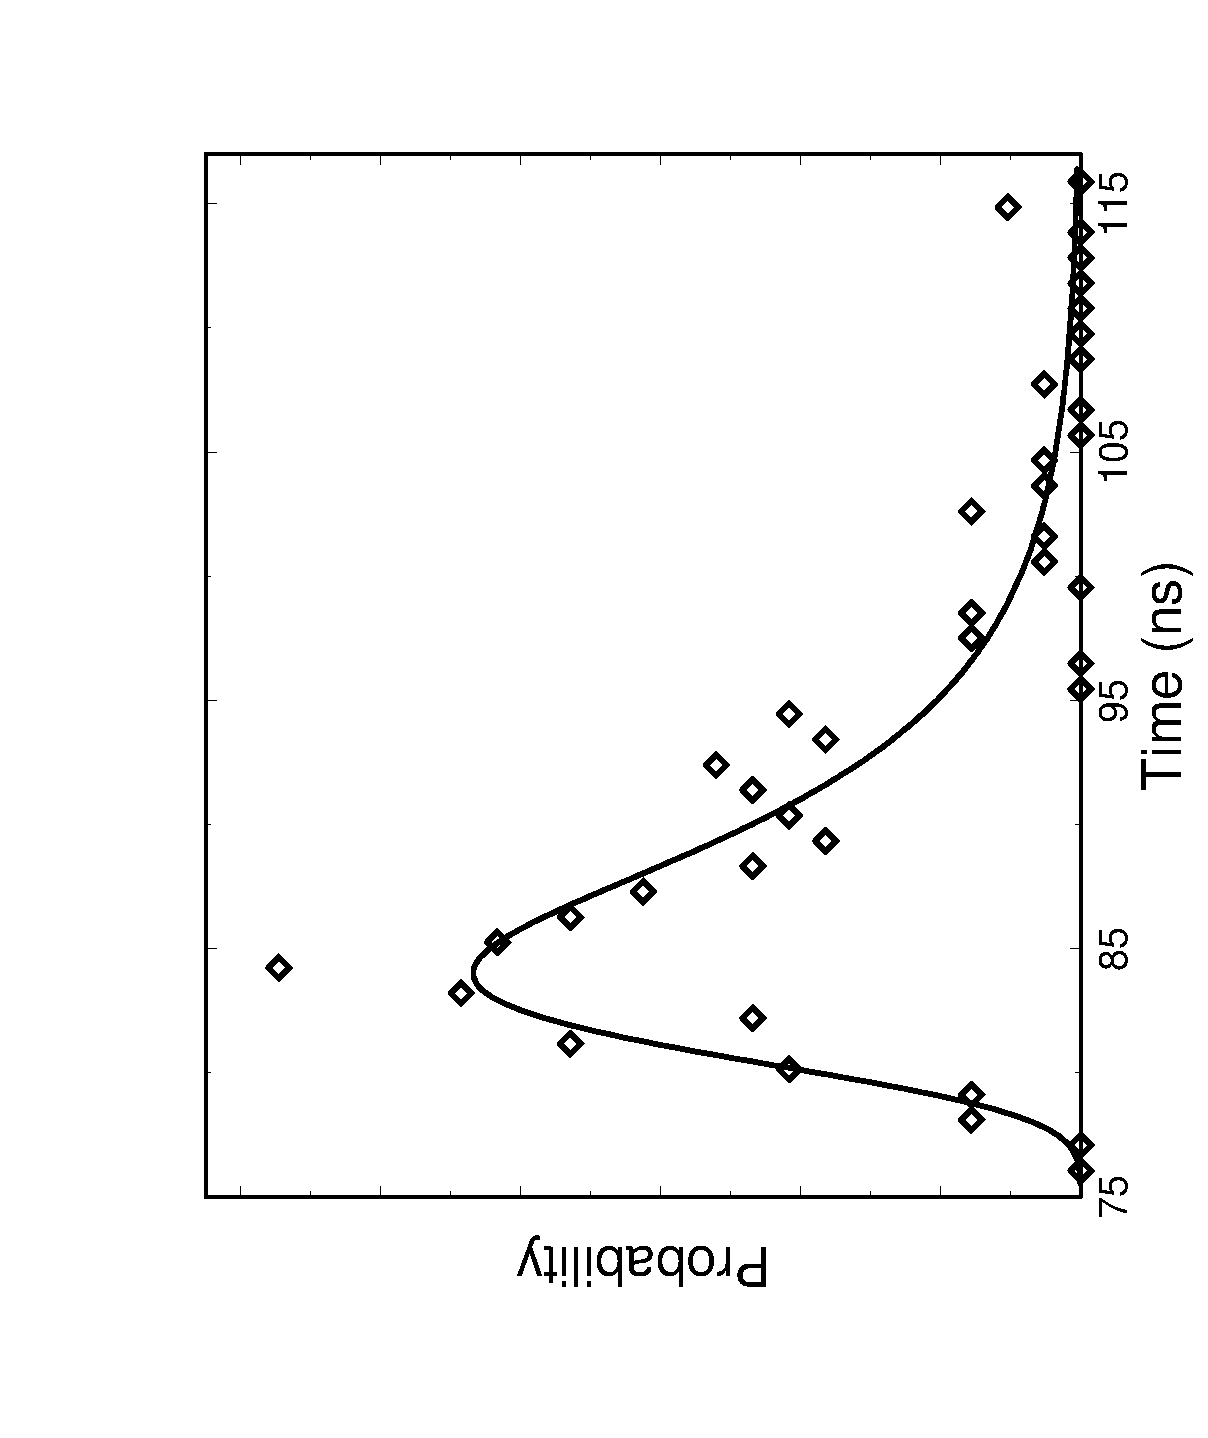
\includegraphics[angle=270,width=8cm]{./graficos/fig_9}
\put(-100,-35){
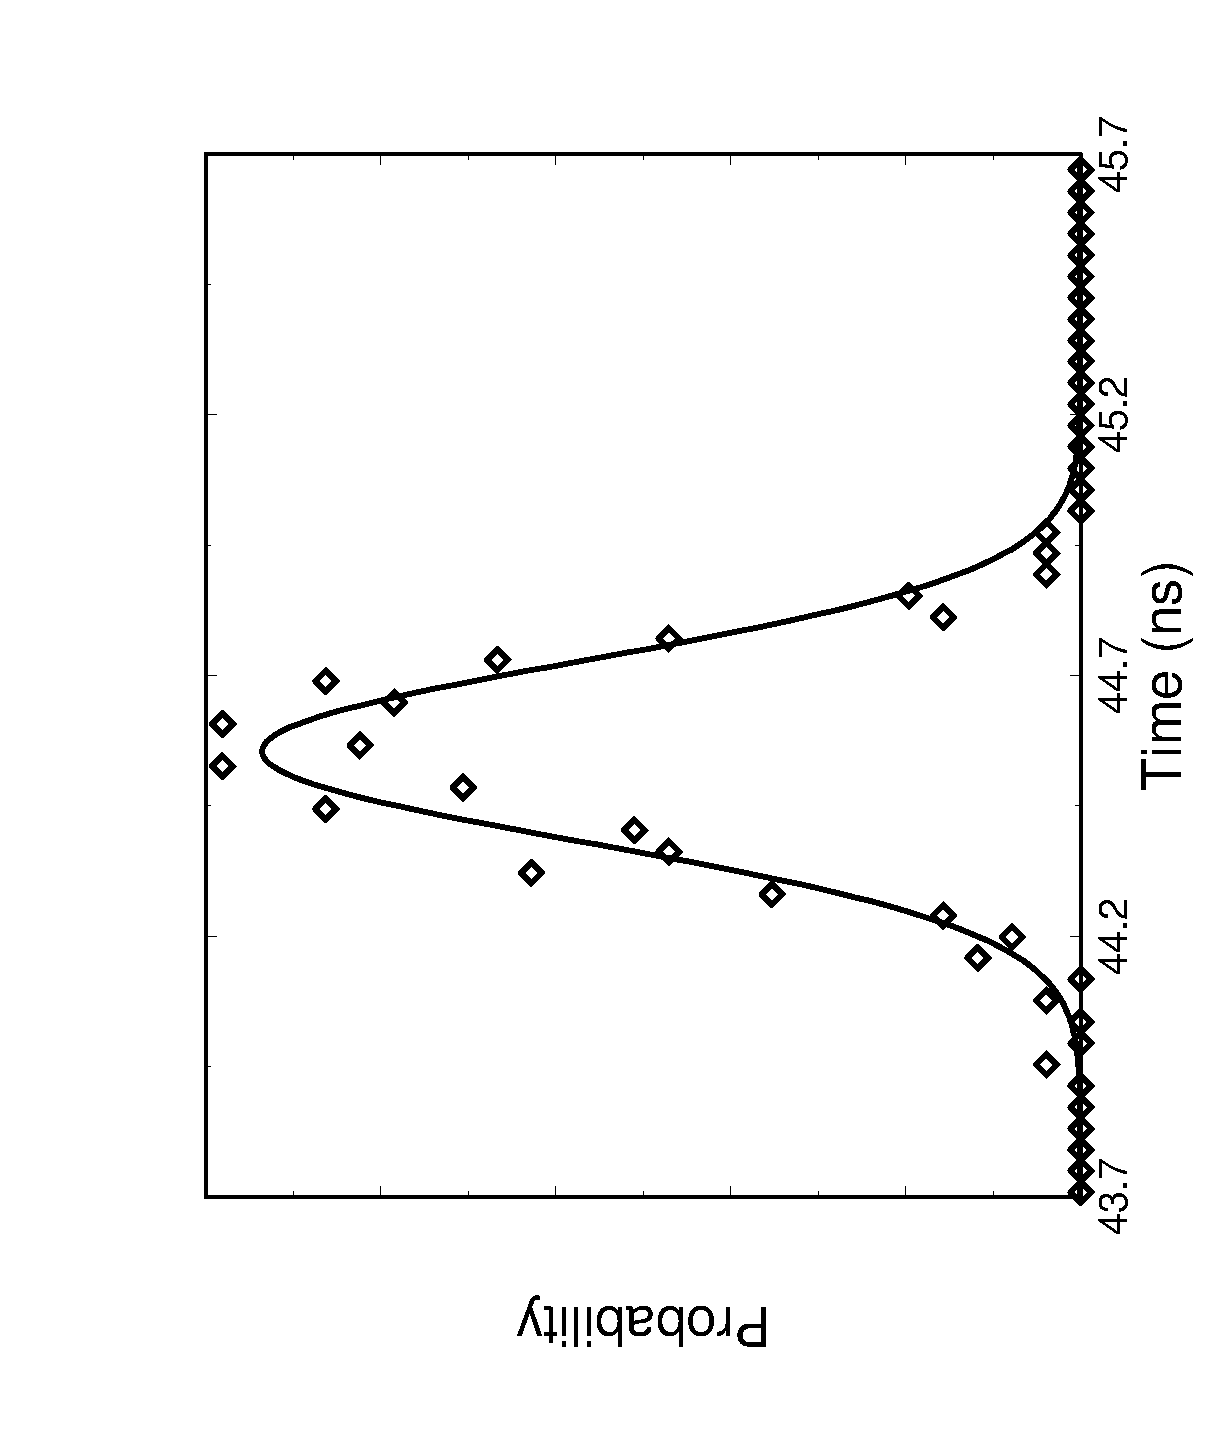
\includegraphics[angle=270,scale=0.1]{./graficos/fig_10}
}
\end{figure}

\end{frame}

%%%%%%%%%%%%%%%%%%%%%%%%%%%%%%%%%%%%%%%%%%%%%%%%%%%%
\begin{frame}[fragile]
\begin{exampleblock}{Ejercicio propuesto 2}
Comprueba que los par\'ametros de comando includegraphics angle y width no son comutativos.
\end{exampleblock}
\begin{figure}
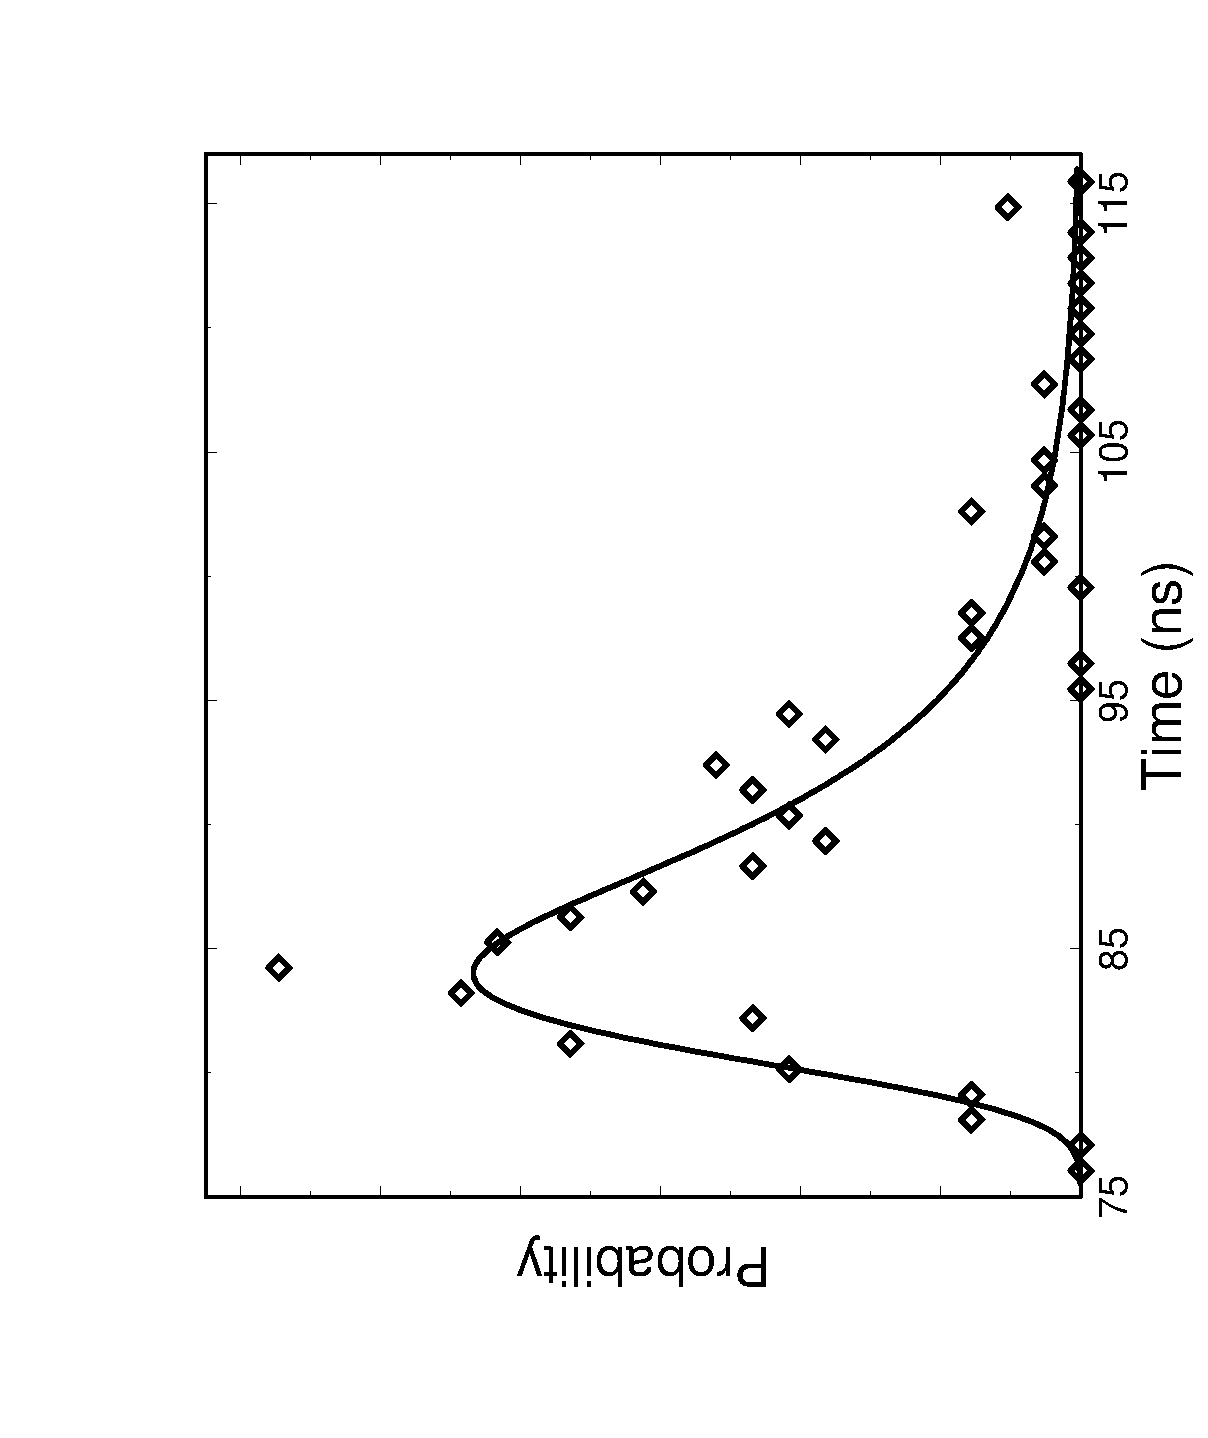
\includegraphics[angle=270,width=4cm]{./graficos/fig_9}
\hspace{0.5cm}
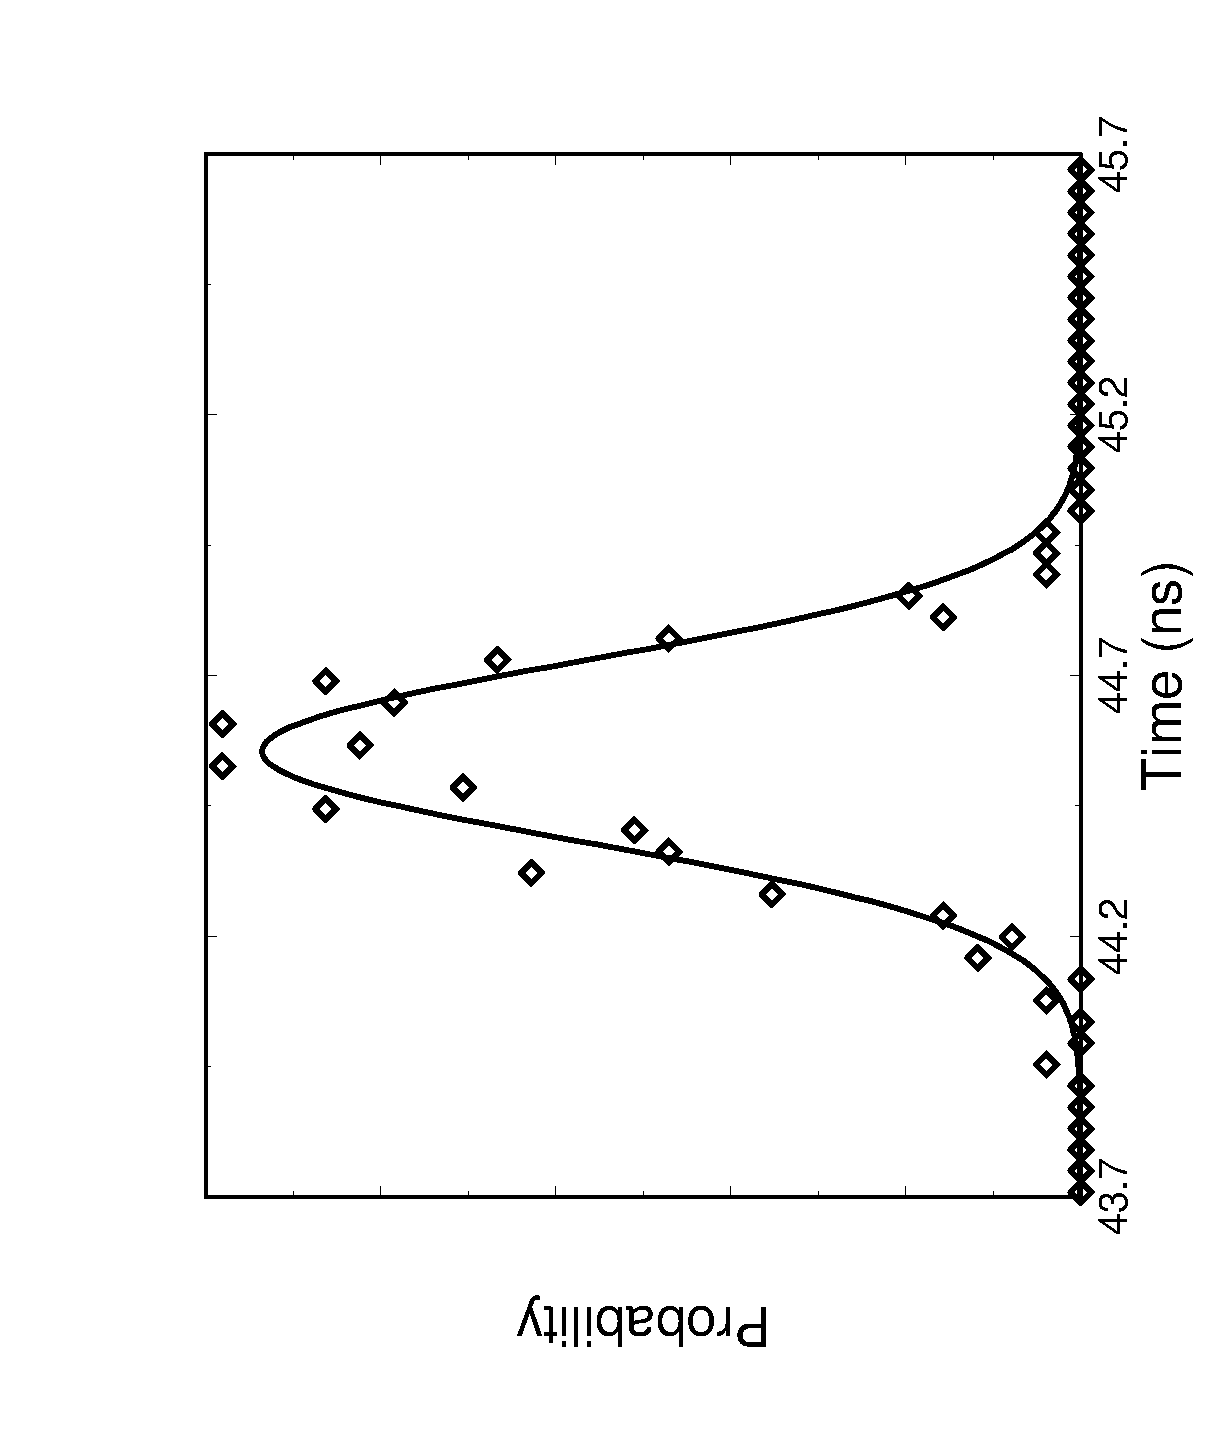
\includegraphics[width=4cm,angle=270]{./graficos/fig_10}
\end{figure}

\end{frame}


%%%%%%%%%%%%%%%%%%%%%%%%%%%%%%%%%%%%%%%%%%%%%%%%%%%%
\begin{frame}[fragile]
\begin{exampleblock}{Ejercicio propuesto 3}
Recorta  y agranda  la niña de la imagen reflejada.
\end{exampleblock}
\begin{figure}
\includegraphics[width=5cm]{./graficos/sorpresa}
\hspace{0.5cm}
\includegraphics[trim = 50mm 0mm 190mm 40mm, clip,width=5cm]{./graficos/sorpresa}
%trim = <left> <lower> <right> <upper>,
\end{figure}


\end{frame}

%%%%%%%%%%%%%%%%%%%%%%%%%%%%%%%%%%%%%%%%%%%%%%%%%%%%
\begin{frame}[fragile]
\begin{exampleblock}{Ejercicio propuesto 4}
Realiza con \LaTeX \ un montaje inspirándote en el siguiente
\begin{figure}
\includegraphics[trim = 50mm 0mm 190mm 40mm, clip,width=5cm]{./graficos/sorpresa}
\hspace{-0.13cm}
\reflectbox{
\includegraphics[trim = 50mm 0mm 190mm 40mm, clip,width=5cm]{./graficos/sorpresa}
}
\put(-210,110){{\color{green}  \LARGE Powered by \LaTeX}}
\end{figure}
\end{exampleblock}
\end{frame}


%%%%%%%%%%%%%%%%%%%%%%%%%%%%%%%%%%%%%%%%%%%%
\begin{frame}[fragile]{Bibliograf\'ia}
\begin{thebibliography}{10}
\bibitem{ManualLatexWikilibros} \href{http://es.wikibooks.org/wiki/Manual_de_LaTeX/Insertar_figuras_en_un_documento}{Manual de Latex/ Insertar figuras en un documento- Wikilibros.}

\bibitem{ManualImportingGraphics}\href{http://en.wikibooks.org/wiki/LaTeX/Importing_Graphics}{Latex/Importing Graphics-Wikilibros.}

\bibitem{DocGraphicx}\href{http://texdoc.net/texmf-dist/doc/latex/graphics/graphicx.pdf}{Documentaci\'on del paquete graphicx}

\bibitem{wrapfigure} \href{http://www.ctan.org/pkg/wrapfig}{P\'agina del paquete wrapfig, ctang.org}

\end{thebibliography}
\end{frame}




\end{document}